\documentclass[fleqn,leqno,10pt,letterpaper,draft]{article}
%----README----
% This TeX file was automatically generated by GNU Emacs's Org Mode.
% For better documentation refer to the corresponding Org file, 
% which you can find in the sources specified bellow.
% Do keep in mind that this file undergoes little to none manual revision.
%----LICENSE---
% Copyright 2021 Jhonny Lanzuisi (jalb97@gmail.com)
% More source files at github.com/JLanzuisi
%
% This program is free software: you can redistribute it and/or modify
% it under the terms of the GNU General Public License as published by
% the Free Software Foundation, either version 3 of the License, or
% (at your option) any later version.
%
% This program is distributed in the hope that it will be useful,
% but WITHOUT ANY WARRANTY; without even the implied warranty of
% MERCHANTABILITY or FITNESS FOR A PARTICULAR PURPOSE.  See the
% GNU General Public License for more details.
%
% You should have received a copy of the GNU General Public License
% along with this program.  If not, see <https://www.gnu.org/licenses/>.
%--------------

\hfuzz1pc
\overfullrule=2cm

\usepackage[spanish,es-noindentfirst]{babel}
\usepackage{csquotes}

\usepackage
[
	includehead,
	includefoot,
	top=.5cm,
	bottom=.5cm,
	left=1.7cm,
	right=7.3cm,
	marginparsep=0.5cm,
	marginparwidth=7cm,
]
{geometry}

\usepackage{mathtools}
\DeclareMathOperator{\Rea}{Re}
\DeclareMathOperator{\Ima}{Im}
\DeclareMathOperator{\car}{car}
\DeclareMathOperator{\traz}{tr}
\DeclareMathOperator{\gen}{gen}
\DeclareMathOperator{\mcm}{mcm}

\usepackage{unicode-math}

\setmainfont{New Computer Modern Book}
\defaultfontfeatures{Scale=MatchLowercase}
\setsansfont{Public Sans}
\setmonofont{Average Mono}
\newcommand{\headfont}{\sffamily}

\frenchspacing
\linespread{1.05}

\setmathfont{New Computer Modern Math}

\usepackage[final]{microtype}

\PassOptionsToPackage{final}{graphicx}
\PassOptionsToPackage{dvipsnames}{xcolor}

\usepackage
{
	xcolor,
	graphicx,
	cancel,
	booktabs,
	hyphenat,
	authoraftertitle,
	pdfpages,
	metalogo
}

\usepackage
[
backend=biber,
backref=true,
citestyle=authoryear-comp,
style=chicago-authordate ,
sorting=ynt
]
{biblatex}
\addbibresource{/home/jhonny/git/Misc-LaTeX-files/bib/general.bib}

\usepackage{url} 
\usepackage{hyperref} 
\definecolor{Carmine}{HTML}{960018}
\newcommand{\linkcolor}{Carmine}
\hypersetup
{
colorlinks=true,
linkcolor=\linkcolor,
urlcolor=\linkcolor,
citecolor=\linkcolor
}
\usepackage[spanish,nameinlink]{cleveref}

\newcommand{\marfont}{}

%\renewcommand*{\marginfont}{\marfont}
\let\oldmarginpar\marginpar
\renewcommand
	{\marginpar}
	[1]
	{
	\oldmarginpar{\raggedright\marfont #1}
	}

\newcounter{nota}
\newcommand
	{\nota}
	[1]
	{
	\refstepcounter{nota}\textsuperscript{\thenota}
	\marginpar{
		\raggedright\itshape\thenota. #1
		}
	}

\renewcommand{\footnote}{\nota}

\usepackage{enumitem} 
\setlist[enumerate]{left=-11pt,nosep}
\setlist[description]{font=\normalfont,leftmargin=\parindent}
\setlist[itemize]{label={\small\textbullet},left=-11pt}

\newcommand{\Asignatura}{}
\newcommand
	{\asignatura}
	[1]
	{\renewcommand{\Asignatura}{#1}}

\makeatletter
\def\@maketitle
	{
	\newpage
	\null
	\let \footnote \thanks
  	\begin{flushleft}\sffamily
  	\marginpar
		{
		\vspace*{.2em}
		\begin{minipage}{.7\marginparwidth}
		\begin{center}
		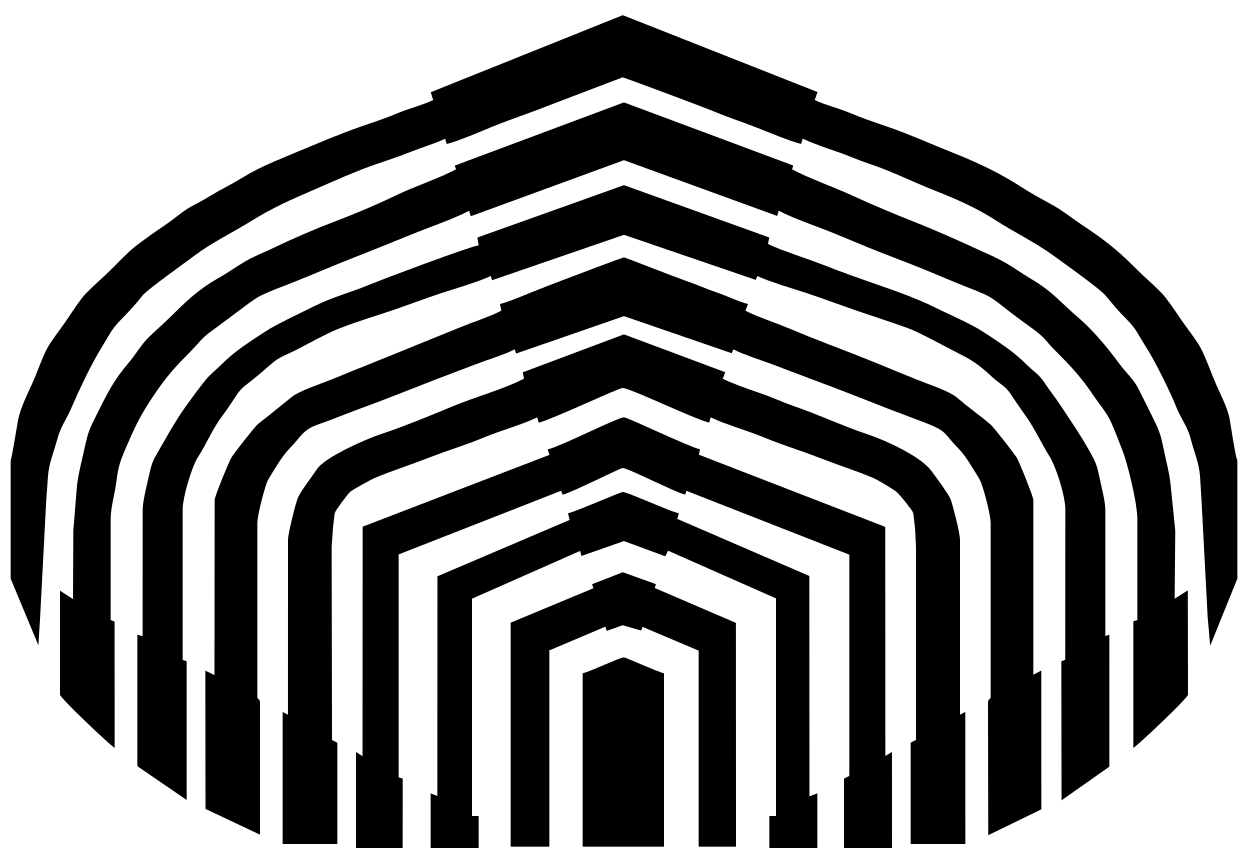
\includegraphics
			[width=.35\marginparwidth]
			{/home/jhonny/git/LaTeX-University/usb-logo.png}\\
		Universidad Simón Bolívar\\
		Caracas, Venezuela\\
		\end{center}
		\end{minipage}
		}
	{
	\Large\headfont
		\MyTitle
	\par
	}
	\smallskip
	\Asignatura\par
	\smallskip
	\@author,\ \today.
	\end{flushleft}
	\vskip 1.5\baselineskip
	}
\makeatother

\usepackage[final]{listings} 
\lstset
{
numbers=left, numberstyle=\tiny\ttfamily, stepnumber=2, numbersep=5pt, 
basicstyle=\ttfamily, 
stringstyle=\ttfamily,
commentstyle=\itshape,
breaklines=true,
postbreak=\mbox{$\hookrightarrow$\enspace},
columns=flexible
}

\usepackage{caption} 
\captionsetup
{
font={rm},
justification=raggedright,
singlelinecheck=false,
skip=3pt
}

\usepackage[explicit]{titlesec}

\titleformat{\section}[hang]
	{\flushleft\headfont}
	{\addfontfeatures{Numbers=Lining}\thesection}
	{1em}
	{\addfontfeatures{LetterSpace=5}\MakeUppercase{#1}}
	[]
\titlespacing*{\section}
	{0em}
	{1.5\baselineskip}
	{.5\baselineskip}
\titleformat{\subsection}
	{\flushleft\sffamily}
	{\addfontfeatures{Numbers=Lining}\thesubsection}
	{.5em}
	{#1}
	[]
\titlespacing*{\subsection}
	{0em}
	{1\baselineskip}
	{1\baselineskip}
\titleformat{\paragraph}[runin]
	{\scshape}
	{}
	{0em}
	{\MakeLowercase{#1}}
	[.]
\titlespacing*{\paragraph}
	{0em}
	{1\baselineskip}
	{5pt}

\let\oldtoc\tableofcontents
\renewcommand
{\tableofcontents}
{\marginpar{\bigskip\oldtoc}}
\usepackage{titletoc}

\titlecontents{section}
	[0em]
	{\vspace{0pt}}
	{\contentsmargin{0pt}}
	{\contentsmargin{0pt}}
	{\contentspage}
	[\vspace{.3em}]
\titlecontents{subsection}
	[1.5em]                              
	{\vspace{0pt}}
	{\contentsmargin{0pt}\small}
	{\contentsmargin{0pt}\small}        
	{\small\contentspage}                 
	[\vspace{.3em}]

\usepackage{fancyhdr}

\renewcommand{\headrulewidth}{0pt}
\setlength{\headheight}{14pt}

\pagestyle{fancy}
\fancyhf{}
\fancyhead
	[L]
	{
	\ifodd\value{page}\MyTitle\else\Asignatura\fi
	}
\fancyhead[R]{\thepage}
\fancypagestyle
	{plain}
	{
	\fancyhead[R]{}
	\fancyhead[L]{}
	\fancyfoot[R]{}%
	\fancyfoot[L]{}
	\fancyfoot[C]{}
	}

\usepackage[thmmarks]{ntheorem}
  % \usepackage[thmmarks]{ntheorem}
  % 	\theoremstyle{plain}
  % 	\theoremindent0cm
  % 	\theorempreskip{0cm}
  % 	\theorempostskip{0cm}
  % 	\theoremheaderfont{\hspace*{\parindent}\upshape}
  % 	\theorembodyfont{\itshape}
  % 	\theoremseparator{.}
  % 	\newtheorem{teo}{Teorema}[section]
  % 	\newtheorem{cor}{Corolario}[teo]
  % 	\newtheorem{prop}{Proposición}[section]
  % 	\newtheorem{lem}{Lema}[section]
  % 	\theoremstyle{nonumberplain}
  % 	\theoremheaderfont{\normalfont}
  % 	\theorembodyfont{\upshape}
  % 	\newtheorem{proof}{Demostración}
  % 	\theoremstyle{plain}
  % 	\theorempreskip{1em}
  % 	\theorempostskip{1em}
  % 	\theoremheaderfont{\upshape}
  % 	\theorempostwork{\noindent}
  % 	\newtheorem{definition}{Definición}[section]

\theoremstyle{plain}
\theorempreskip{\medskipamount}
\theorempostskip{\medskipamount}
\theorembodyfont{\upshape}
\theoremseparator{.}
{
\theoremheaderfont{\itshape}
\newtheorem{definition}{Definición}
}
{
\theoremheaderfont{\scshape}
\newtheorem{theorem}{Teorema}
}


\title{Tercer Ejercicio}
\author{Jhonny Lanzuisi, 15\,10759}
\asignatura{Universidad Simon Bolivar, Topología 1}

\begin{document}
\maketitle
\tableofcontents
\marginpar{
	\begin{abstract}
		 \Asignatura, Tercera tarea. Espacios topológicos, bases, comparación de topologías y ordenes parciales. 
	\end{abstract}
}

\section[Enunciado]{Enunciado}

Sea $X$ un conjunto ordenado parcialmente. Sean $U_L(x)=\left\{ y\mid y\prec x \right\}$ y
$U_R(x)=\left\{ y\mid x\prec y \right\}$. \textit{Demuestre que:} 
\begin{enumerate}
	\item Las familias $\left\{ U_L(x) \right\}$, $\left\{ U_R(x) \right\}$ son bases de dos topologías
	$\mathcal{T}_L$ y $\mathcal{T}_R$, respectivamente, sobre $X$.
	\item $G$ esta en $\mathcal{T}_L$ si, y solo si, se cumple que 
		\[
			x\in G\implies U_L(x)\subset G.
		\]
	\item En $\mathcal{T}_L$ las intersecciones arbitrarias de conjuntos abiertos
		dan conjuntos abiertos.
	\item La topología discreta es la única mas fina que $\mathcal{T}_L$ y $\mathcal{T}_R$.
	\item Las topologías $\mathcal{T}_L$ y $\mathcal{T}_R$ no son comparables. 
\end{enumerate}

\section{Solución}

\paragraph{Parte 1}%

Primero veamos que las familias $\left\{ U_L(x) \right\}$, $\left\{ U_R(x) \right\}$
cubren el conjunto $X$. Esto no es muy complicado puesto que, para todo $x\in X$,
los conjuntos $ U_L(x) $ y $ U_R(x) $ contienen a $x$ 
(debido a la reflexividad de $\prec$) de donde se sigue que $X$ puede escribirse
como la unión de los $U_L(x)$ o como unión de los $U_R(x)$.

Tomemos ahora un elemento $y_1$ en $U_L(x_1)\cap U_L(x_2)$, donde
$x_1,x_2$ son elementos de $X$. Entonces
\[
	y_1\in U_L(y_1),
\]
por la misma razón que antes, y
\[
	U_L(y_1)\subset U_L(x_1)\cap U_L(x_2)
\]
puesto que si tomamos un $y\in U_L(y_1)$ entonces $y\prec y_1$, pero como
$y_1\prec x_1$ y $y_1\prec x_2$, se tiene que $y\prec x_1$ y $y\prec x_2$ por
transitividad. Hemos descubierto que para todo elemento en la intersección de dos $U_L$
podemos conseguir otro conjunto $U_L$ tal que contiene a dicho elemento y esta contenido en la
intersección, es decir, que la familia $\left\{ U_L(x) \right\}$ forma una base para una topología
sobre $X$ por el teorema~\ref{teo1}. Esta topología es $\mathcal{T}_L$.

Un argumento análogo al anterior nos da como resultado que la familia $\left\{ U_R(x) \right\}$ también es
base de una topología sobre $X$, y esta topología es $\mathcal{T}_R$.

\paragraph{Parte 2}
Supongamos que $G$ pertenece a $\mathcal{T}_L$, entonces $G$ se escribe como una unión arbitraria
de elementos básicos, es decir, 
\begin{align}
	G = \bigcup_\alpha U_L(x_\alpha).\label{eq1}
\end{align}
Si tomamos un $x\in G$ se sigue que $x$ debe pertenecer a alguno de los $U_L(x_\alpha)$. Como $x$ pertenece
a este elemento básico se tiene que $x\prec x_\alpha$ pero entonces, por definición de los $U_L$,
\[
	U_L(x)\subset U_L(x_\alpha)
\]
y por la igualdad en~\ref{eq1},
\[
	U_L(x)\subset U_L(x_\alpha)\subset G
\]
de donde se tiene, claramente, que $U_L(x)\subset G$.

Supongamos ahora que para cada $x\in G$ se cumple que
\[
	x\in G\implies U_L(x)\subset G.
\]
Pero como $U_L(x)$ es un elemento de la base de $\mathcal{T}_L$, la implicación anterior
da de forma inmediata, por el teorema~\ref{teo2}, que $G\in\mathcal{T}_L$.

\paragraph{Parte 3}%

Sea $\mathcal{A}=\left\{ A_\alpha\mid\alpha\in\mathscr{A} \right\}$ una familia de conjuntos abiertos
de $\mathcal{T}_L$, y consideremos la intersección
\[
	\bigcap\mathcal{A}.
\]

Si tomamos un $x\in\cap\mathcal{A}$ entonces $x$ pertenece a todos los $A_\alpha$. Como estos conjuntos
$A_\alpha$ son abiertos se sigue, por la parte anterior, que $U_L(x)$ esta contenido en todos
los $A_\alpha$. Pero esto es lo mismo que decir que
\[
	U_L(x)\subset\bigcap\mathcal{A},
\]
y, nuevamente por la parte anterior, se tiene que $\cap\mathcal{A}$ es un conjunto abierto. 

\paragraph{Parte 4}%

Sea $\mathcal{T}$ una topología sobre $X$ tal que
\begin{align}\label{eq2}
	\mathcal{T}_L\subset\mathcal{T}\quad\text{y}\quad\mathcal{T}_R\subset\mathcal{T}.
\end{align}
Sabemos que al menos una tal $\mathcal{T}$ existe: la topología discreta, a la que llamaremos $\mathcal{D}$, por lo que
tiene sentido preguntarse si existe otra topología con esta propiedad.

Veamos. Dado cualquier $x\in X$, la topología $\mathcal{T}$ debe cumplir (por~\ref{eq2})
\[
	U_L(x)\in\mathcal{T}\quad\text{y}\quad U_R(x)\in\mathcal{T}.
\]

Pero como $\mathcal{T}$ es una topología la intersección $U_L(x)\cap U_R(x)=\left\{ x \right\}$ debe pertenecer también a $\mathcal{T}.$
Entonces todos los conjuntos de la forma $\left\{ x \right\}$ ($x\in X$) pertenecen a $\mathcal{T}$, es decir, $\mathcal{D}\subset\mathcal{T}$.

Pero como $\mathcal{D}$ siempre es la topología mas fina, se tiene también $\mathcal{T}\subset\mathcal{D}$, por lo que
$\mathcal{D}=\mathcal{T}$.

Es decir, $\mathcal{D}$ es la única topología más fina que $\mathcal{T}_L$ y $\mathcal{T}_R$.
\paragraph{Parte 5}%

Notemos primero que se puede establecer un criterio análogo al de la parte 2
para caracterizar los conjuntos abiertos de $\mathcal{T}_R$, y la demostración de este hecho
es muy parecida a la de la parte 2.

Tomemos dos elementos $x_1,x_2$ de $X$ tales que $x_1\prec x_2$. Entonces el cojunto $U_L(x_1)$, que
es abierto en $\mathcal{T}_L$, \emph{no contiene} a ningun elemento $y$ que suceda a $x_1$ (por ejemplo,
no contiene a $x_2$) por lo que $U_R(x_1)\not\subset U_L(x_1)$ y por lo tanto $U_L(x_1)$ no es abierto
en $\mathcal{T}_R$. Un ejemplo análogo nos dará un conjunto abierto en $\mathcal{T}_R$ que no es abierto
en $\mathcal{T}_L$. Entonces se tiene que $\mathcal{T}_L\not\subset\mathcal{T}_R$ y $\mathcal{T}_R\not\subset\mathcal{T}_L$.

\section[Resultados Utilizados]{Resultados Utilizados}%
\label{sec:resultados_utilizados}

\begin{teo}\label{teo1}
	Sea $\mathcal{B}=\left\{ U_\alpha \mid \alpha\in \mathscr{M} \right\}$ una familia de subconjuntos de $X$
	que cubre a $X$ y satisface la siguiente condición:
	\begin{itemize}
		\item 	Para cada $\alpha,\beta\in\mathscr{M}\times\mathscr{M}$ y cada $x\in U_\alpha\cap U_\beta$,
	existe un $U_\gamma$ tal que $x\in U_\gamma\subset U_\alpha\cap U_\beta$.
	\end{itemize}
	
	Entonces el conjunto $\mathcal{T}(\mathcal{B})$ que consiste de $X,\emptyset$ y todas las uniones de miembros
	de $\mathcal{B}$ es una topología sobre $X$, es decir, $\mathcal{B}$ es la base de \emph{alguna}
	topología sobre $X$.
\end{teo}

\begin{teo}\label{teo2}
	Sea $\mathcal{B}\subset\mathcal{T}$ una base para la topología $\mathcal{T}$. Entonces un conjunto $A$
	es abierto (es decir, pertenece a $\mathcal{T}$) si, y solo si, para cada $x\in A$ existe un
	$U\in\mathcal{B}$ tal que $x\in U\subset A$.
\end{teo}

\printbibliography[
heading=bibintoc,
title={Referencias}
]
\end{document}
